\documentclass[oneside]{book}
% % % % % % % % % % % % % % % % % % % 
%
%  USEPACKAGES; kept minimal, these can be amended but not removed.
%
% % % % % % % % % % % % % % % % % % %
\usepackage{fancyhdr}
\usepackage{pdfpages}
\usepackage{graphicx}
% % % % % % % % % % % % % % % % % % %
% 
% DEFINITIONS FILE
% Change Values of commands in file: "definitions-thesis.tex"
%
% % % % % % % % % % % % % % % % % % %
\newcommand{\studentNumber}{M00000000}
\newcommand{\authorName}{Ian Mitchell}
\newcommand{\thesisTitle}{Challenges to Cyber Security}
\newcommand{\degreeTitle}{BSc (Hons) Cyber Security \& Digital Forensics} 
\newcommand{\moduleCode}{CST3590}
\newcommand{\moduleTitle}{Individual Project}
\newcommand{\moduleLeader}{Dr Xiaochun Chen }
\newcommand{\supervisor}{S. Hara}
\newcommand{\deptName}{Dept. of Computer Science}
\newcommand{\academicYear}{2020-21}


\begin{document}
\frontmatter
% % % % % % % % % % % % % % % % % % %
% 
%	TITLEPAGE - DO NOT CHANGE
%
% % % % % % % % % % % % % % % % % % %
\begin{titlepage}
\begin{center}
	
	
\includegraphics[scale=0.75]{mdxlogo} 
	
	\vfill

	 \begin{tabular}{rl}
	 Module Title: & \moduleTitle\\
	 Module Code:  & \moduleCode\\
	 Module Leader:& \moduleLeader\\
	 \end{tabular}
	
	\vfill

			{\huge \thesisTitle \\}

	\vfill

	\begin{tabular}{rl}
	Student: &	\authorName \\
	Student Number: & \studentNumber  \\
	Supervisor: & \supervisor \\ 
	\end{tabular}
	\vfill
	
	A thesis submitted in fulfilment of the requirements\\ for the degree of \degreeTitle
	\vfill
	\deptName 
	\vfill
	\academicYear
\end{center}

\end{titlepage}
\newpage

% % % % % % % % % % % % % % %
%
%	DECLARATION PAGE - 
%	DO NOT EDIT
% % % % % % % % % % % % % % %
\chapter*{Declaration}
\noindent I, \authorName, declare that this thesis titled, ``\thesisTitle" and the work presented in it are my own. I confirm that:

\begin{itemize} 
\item This work was done wholly for a degree at Middlesex University.
\item Where any part of this thesis has previously been submitted for a degree or any other qualification at Middlesex University or any other institution, this has been clearly stated.
\item Where I have consulted the published work of others, this is always clearly attributed.
\item Where I have quoted from the work of others, the source is always given. With the exception of such quotations, this thesis is entirely my own work.
\item I have acknowledged all main sources of help.
\item Where the thesis is based on work done by myself jointly with others, I have made clear exactly what was done by others and what I have contributed myself.\\
\end{itemize}
 
\noindent Signed:\\
\rule[0.5em]{25em}{0.5pt} % This prints a line for the signature
 
\noindent Date:\\
\rule[0.5em]{25em}{0.5pt} % This prints a line to write the date
\addcontentsline{toc}{section}{Declaration}
\newpage

% % % % % % % % % % % % % % %
%
%		ABSTRACT
%		EDIT
% % % % % % % % % % % % % % %
\chapter*{Abstract}
The Thesis Abstract is written here (and usually kept to just this page). The page is kept centred vertically so can expand into the blank space above the title too \ldots
\addcontentsline{toc}{section}{Abstract}


% % % % % % % % % % % % % % % %
%
%			AKNOWLEDGEMENTS
%			EDIT
% % % % % % % % % % % % % % % %
\chapter*{Acknowledgements}
The acknowledgements and the people to thank go here, don't forget to include any support you may have received from family and friends \ldots
\addcontentsline{toc}{section}{Acknowledgements}
\newpage
\tableofcontents


\mainmatter
% % % % % % % % % % % % % % % % % %
%
%		HEADERS & FOOTERS
%		DO NOT EDIT
% % % % % % % % % % % % % % % % % % %
\pagestyle{fancy}
\rhead{Chapter \thechapter}
\lhead{\studentNumber}
\lfoot{\empty}
\cfoot{\thepage}
\rfoot{\empty}


% % % % % % % % % % % % % % % %
%
% CONTENT
% EDIT
% % % % % % % % % % % % % % % %
\chapter{Proposal}
\section{Introduction}
Include a few words here about the background and motivation of the project. 

This can be helped by explaining what has happened in the past; what you are going to do in the present; and how this action will help and change the future. 



\section{Aims}
This should be a general aim of the overall project. This should be explained in one or two paragraphs.

\subsection{Objectives}
These are a list of clearly defined objectives that can be aligned to outcomes in the project. We can define the success of the project based on these fulfilling these objectives.
\begin{itemize}
\item Research
\item Explore Hypotheses
\item Design Experimental Framework
\item Run experiments under Experiment Framework and test hypotheses
\item Analyse Results
\item Provide detailed recommendations and guidelines 
\end{itemize}


\subsection{Deliverables}
Deliverables are a result of actions that complete and attempt to satisfy objectives and can include:
\begin{itemize}
\item Complete proposal
\item Complete Research Ethics approval
\item Complete research on specified related area
\item Complete research on another specified related area
\item Complete Literature Review
\item Conduct Experiments under completed Designed Experimental Framework
\item Complete Software Development
\item Complete Experiments based on Experimental Framework
\item Collate and gather information and data from Experiments
\item Analyse Results and complete write-up of results
\item Complete Conclusions
\item Complete Turn-it-in submission
\item Print, bind and submit two hard copies to Unihelpdesk.
\end{itemize}

\section{Resources}
List any software or hardware that may be required for the completion of the project.

\begin{itemize}
\item Forensic ToolKit
\item The Sleuth Kit
\item Laptop
\item 10 1Gb memory sticks
\item 2 128Gb SSD
\item FTK Imager
\end{itemize}

\section{Schedule}
Typically include a GANTT chart indicating when the objectives and deliverables are met.

This can be completed by Excel or other dedicated software and then imported into this document as shown in Fig.\ref{fi:GANTT}.

\begin{figure}
\centering
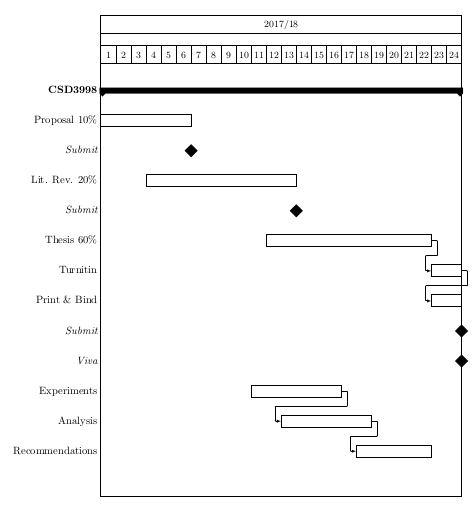
\includegraphics[scale=0.4]{gantt}
\caption{GANTT Chart showing indicative milestones.}\label{fi:GANTT}
\end{figure}


\section{Summary}

Optional, but this section could outline and emphasise the structure of the thesis. It could also be used to emphasise what the project is about and can sometimes be used to disambiguate any areas, e.g., your project may look into applying text mining to e-discovery and you may want to emphasise that this is an application and not a project on text mining.

The structure of the rest of this thesis (never refer to the thesis as a paper and always write in third person) is as follows: Chapter 2 covers the literature review and current research related to the problem; Chapter 3 investigates the experiment and rationalises the method undertaken; Chapter 4 analyses the results; and Chapter 5 includes the recommendations and conclusions. 



\chapter{Literature Review}
\section{Introduction}
Outlining the main area you are researching. This may also include any motivation for investigation.
\section{Subject}
You can divide your Literature Review into several sections, one for each topic/area you are reviewing.
\subsection{title}
Each subject area will probably be broken down to several subsections.
\subsubsection{title}
It is generally unnecessary to go further than the subsection level, however, in rare circumstances the subsubsection command can be used. 

\section{Citation \& Reference}
Exercises show two there are two parts to a citation: the citation; and the reference. There are many styles and configurations of the citations and references, which the exercises will make clear. 

Essentially, to start with, we are going to keep this simple and use the plain bibliography setting. As we advance the national bibliography package can be used and this is in the exercises on citations. This setting orders all bibliography items in alphabetical order and only uses the cite command. It does have its restrictions and we will come across these and how to cope with them. The following is an example paragraph using citations and a plain bibliography and should be adequate to get us started.


The first generation of Neural Networks are generally considered as Perceptrons \cite{rosenblatt1958perceptron}. Minsky and Papert \cite{minsky1969perceptrons} wrote a critique of the perceptron which showed that it could not solve non-linear problems, typically XOR. To solve the non-linear problem Rumelhart, Hinton and Williams \cite{rumelhart1985learning} made an enormous contribution with the Back-propagation error Artificial Neural Network, ANN. This and related ANN are generally referred to as second generation and inspire many of the techniques used in machine learning. The third generation of neural networks are based on biologically-inspired neurons and are generally referred to as, ``spiking neurons''.  Oddly many third generations are based on research pre-dating to first and second generations, namely Hebbian Learning \cite{Hebb}. These spiking neurons can be built into bigger networks to solve complex problems,e.g., see \cite{huyck2013compensatory}.

\section{Summary}
Conclude on your main findings and how they are going to contribute to solving objectives.

This thesis is an outline and can be deviated from. For example, it would be completely justified to have two Literature Review Chapters, if the subject areas are unrelated and completely separate. Often new research can be considered as two subject areas merged together to form a new area, e.g., text-mining and e-discovery. This would result in two literature review chapters: i) text-mining; and ii) e-discovery. 



\chapter{Method}
\section{Introduction}
Go over the objectives of the experiment relying on new research in your literature review. 
\section{Experiment 1}
Many Experiment Frameworks require two experiments, one with $x$, the other without. These are often referred to as control experiments.

\section{Experiment 2}
All experiments are repeated for reproducibility, you need to show how each stage of the experiment is designed to help prove or disprove your hypothesis. 

\section{Summary}
You have no results, however, you have a clear and concise experiment to run. With your knowledge from Literature Review you can mention the expected outcomes of each experiment.

\chapter{Analysis \& Results}
\section{Introduction}
Include any set up for the experiment. This could be as follows:
\begin{itemize}
\item Architecture:          x86\_64
\item CPU op-mode(s):        32-bit, 64-bit
\item Byte Order:            Little Endian
\item CPU(s):                4
\item On-line CPU(s) list:   0-3
\item Thread(s) per core:    2
\item Core(s) per socket:    2
\item Vendor ID:             GenuineIntel
\item CPU family:            6
\item Model:                 61
\item CPU MHz:               500.000
\item RAM:					 8Gb
\end{itemize}
\section{Experiment 1}
Use graphics to display results. Most results can be shown in tables. Use package longtables if you have trouble getting all data into a single page. Remember to label and reference the table.

\section{Experiment 2}
Experiment 2 should differ from Experiment 1. Each experiment should be repeated a number of times for reproducibility. Do not confuse Experiment 2 as a repeat of Experiment 1, they are different. 

\section{Summary}
Bad results happen, but it is not bad science. Still write up the results. If given time run more experiments. Rejecting or accepting an hypothesis is still a result worth writing up.

Good results will yield a clear direction and give clear recommendations and guidelines that can be mentioned here and emphasised in the next chapter \-- it is OK to repeat.


\chapter{Conclusions}
Usually the weakest chapter, but the most important. This is where you state your main contribution. Computer Science and Computer Forensics is unlike many other topics, you can become an expert in a small area of computing, say FAT file systems in a matter of months. What you are studying, not only should you enjoy, but you should be an expert in. In Medicine it could take 20 years to be an expert in some field. 

Have all you aims and objectives been met, if so where and how did you prove them?



\section{Recommendations}
This expertise should leave you to some insight and recommendations based on your knowledge of the subject and your results. These are mentioned here. 

\section{Future Work}
Any new areas this research could lead to.


\section{Reflections}
How would you complete this project again?

\section{Summary}
Odd to have a summary in a chapter entitled conclusion, however, the purpose of this is to end on a high note. Your reader will have been examining and assessing this thesis for some time and you need to finish it on a high note. Make it succinct and punchy. You should include: the aims and objectives; the hypothesis; any outcomes; any development; accept or reject hypothesis; results; any recommendations; and finally your main contribution.


% % % % % % % % % % % % % % % %
%
% BIBLIOGRAPHY 
% Use basic BiBTex options
%
% % % % % % % % % % % % % % % %
\bibliographystyle{plain}
\addcontentsline{toc}{chapter}{Bibliography}
\bibliography{ex1}



\appendix
\part*{Appendices}
\addcontentsline{toc}{part}{Appendices}
\chapter{Code}
\begin{verbatim}
#record
popTL.getPop().record(['spikes'])
popTR.getPop().record(['spikes'])
popRight.getPop().record(['spikes'])
popLeft.getPop().record(['spikes'])
popExp.getPop().record(['spikes'])
\end{verbatim}

\chapter{Meetings with Supervisor}
%include pdf file, "meetings.pdf". 
%The options include only page 1, because it is already a4, it is scale down to 0.75. 
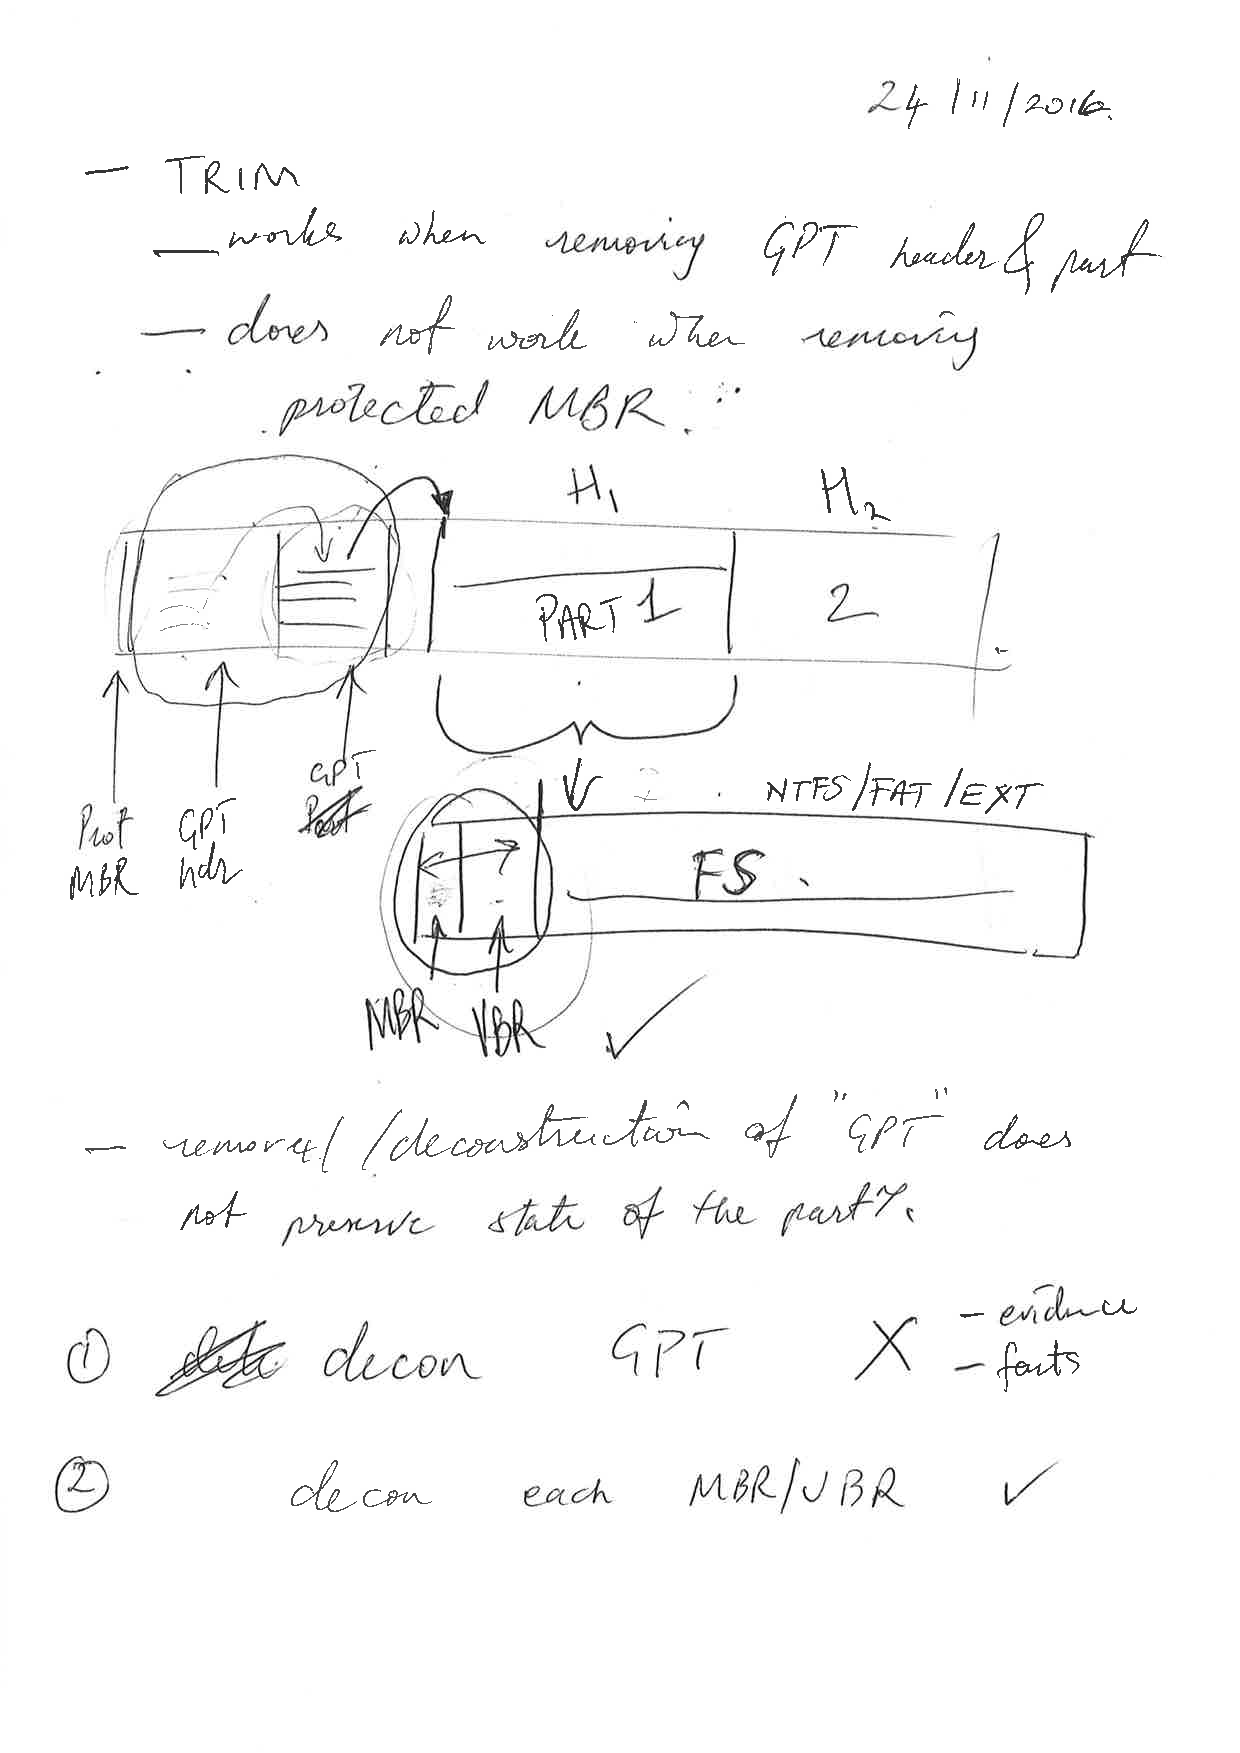
\includepdf[pages=1,scale=0.75]{meetings}




\chapter{Ethical Approval}
\includepdf[pages=6]{meetings}

\end{document}
